\begin{table*}
	\centering
	\begin{tabular}{| c | p{0.25\textwidth}|c |c |c || c |c |c |}
	
	
 	    \multicolumn{2}{c}{} & \multicolumn{3}{c}{Web Traffic} 		  & \multicolumn{3}{c}{File Transfer} \\
 	     \cline{3-8}	
             \multicolumn{2}{c|}{} & CPU 			& Memory (Mb) 		& Throughput (Mbps)	& CPU 		& Memory (Mb)		& Throughput (Mbps) \\\hline   
Settings 1 & client connected to the gateway with ip forwarding &   3.6\% 		& 693 		& 11.461		& 2.7\%		& 708 Mb		& 11.455 \\\hline
Settings 2 & client connected via squid proxy hosted on the gateway   &   52\%        & 692 		& 11.455		& 47\%		& 703 Mb		& 11.450 \\\hline
Settings 3 & client connected to SvNF proxy hosted on the gateway with no rule deployed &   66\%		& 680 		& 11.404		& 54\%		& 707 Mb		& 11.449 \\\hline
Settings 4 & client connected to SvNF proxy hosted on the gateway with 10,000 rules deployed   &   69\%        & 690 		& 11.430		& 56\%		& 704 Mb		& 11.444 \\\hline
	
	            
	\end{tabular}
	\caption{
	OSGi HTTP proxy performance comparison
	\label{tab:perf-comparison}
	}
	
\end{table*}

Section~\ref{sec:migrating} described the role of SvNF deployed on the HG and the server-side infrastructure composed of various vNF: Streamers deployed in POPS, Caching and Transcoding orchestrator and Transcoding vNF deployed in the core.
As our proposal aims at showing how software deployed in a modular HG can play a role in a vNF architecture, our focus for the evaluation is devoted to assessing HG side performance, memory footprint and environement execution. We also used simulation to evaluate the benefits of this system, based on sensible hypotheses from a French SP network.


\subsection{SvNF Evaluation }\label{Testbed}

We deployed the SvNF OSGi bundle in the Apache Karaf OSGi runtime on an PC Engines APU/1C gateway running Debian Jessie. 
The APU/1C gateway is built uppon a low-power AMD Bobcat microarchitecture, with 3 Gigabit Ethernet channels. The gateway connects the test operator and a PC file server.

\begin{figure}
  \begin{center}
    
\includegraphics[width=0.30\textwidth]{fig/testbed.pdf}
  \end{center}
  \caption{ SvNF Performances testbed
    \label{fig:testbed}
  }
\end{figure}	


\begin{figure}
  \begin{center}
    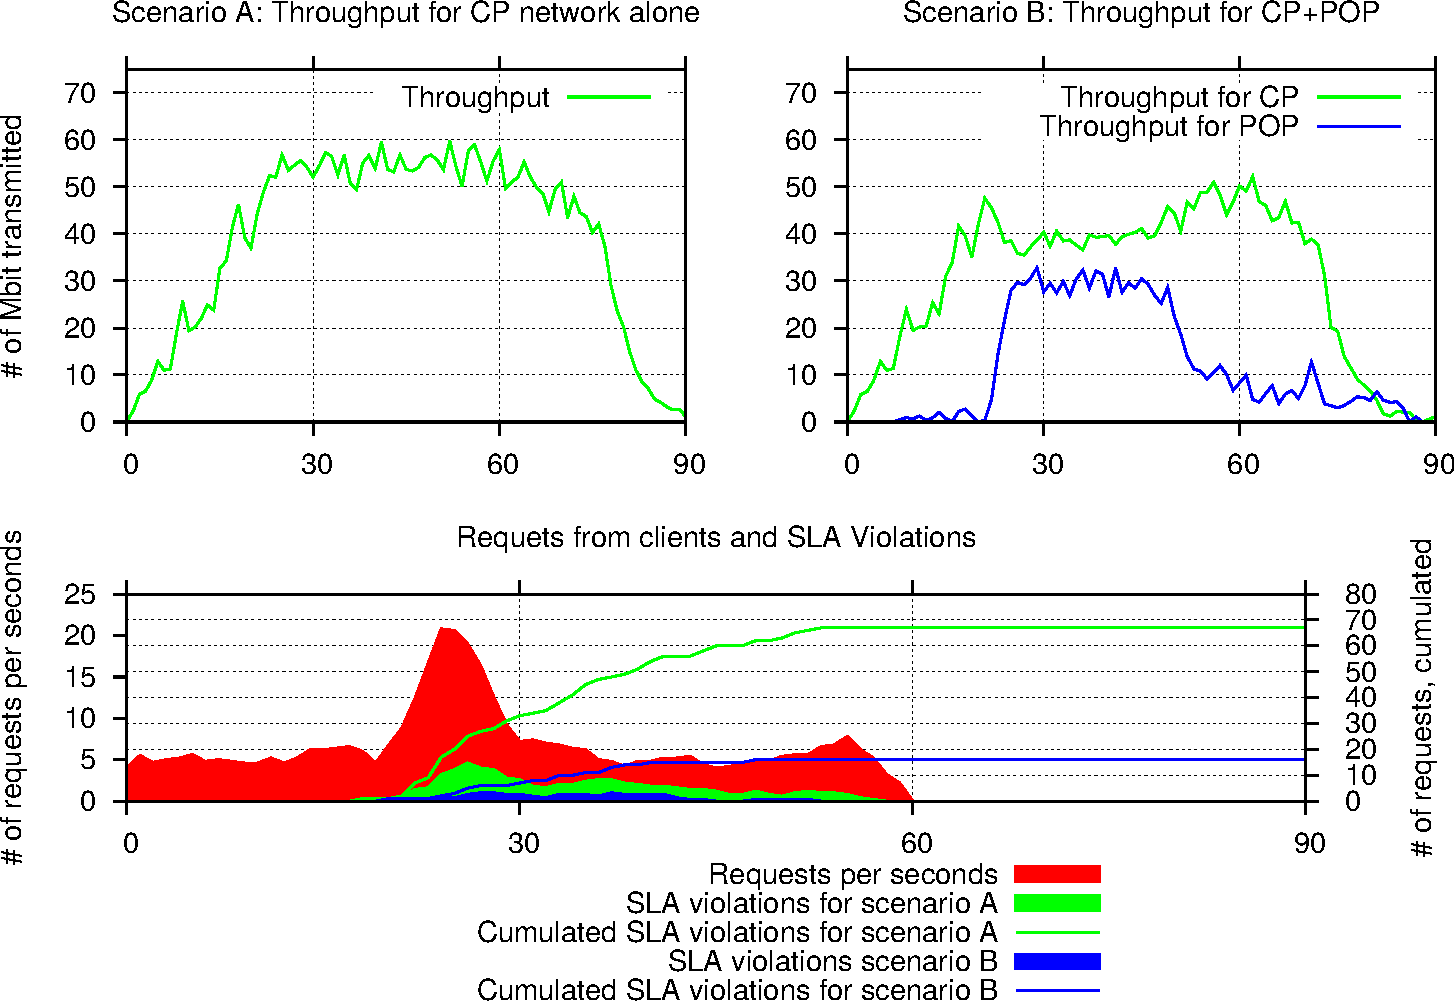
\includegraphics[width=0.5\textwidth]{fig/CP+POP_evaluation.pdf}
  \end{center}
  \caption{ Evaluation of the benefits of the SvNF+vNF system
    \label{fig:cppopeval}
  }
\end{figure}	







JMeter\footnote{http://jmeter.apache.org} was used to capture the network metrics of our solution.
It allowed us to create agents and make them perform standard HTTP queries and report on specific performances metrics. Each experiment consisted of 10 agents continuously downloading target resources on the HTTP file server, 10000 times.

We considered two different validation usecase: Web Traffic and File Transfer. First, the agents were to download a 192 Mb video file, then a single HTML page which linked to 171 static resources composed of Javascript files, CSS and images of average size 16 kb.

We evaluated our solution with two different rules settings deployed in the SvNF. In the first one, we didn't deploy any rule, assessing only the overhead linked to the application network framework. In the second one however, we deployed 10.000 rules, causing the SvNF to process both requests and responses wrt those rules thereby assessing its ability to perform pattern matching in a timely manner. Both cases reflect the no operation scenario presented in ~section \ref{noop}.

We decided to assess the overhead caused the SvNF by comparing it to the well-known Squid3 HTTP proxy. To have a better grasp of the amont of resources consumed by the SvNF, we also reported CPU and memory consumption for each settings as well.

From ~Table \ref{tab:perf-comparison} we can see that the performances in term of throughput is globally the same across all settings, with the maximum deviation from the baseline settings 1 being less that 0.3\%.
In settings 2-4, we also see that a significant share of CPU power is dedicated to processing the resquests for both Squid3 and the SvNF, with the SvNF consuming up to a 25\% extra CPU time, but with no drop in performances. This can be explained by the fact that the SvNF runs on top of a JVM, while Squid is a native application.

As this experiment doesn't intend to mimic real life internet usages but to stress the system up the its limits, we conclude that even with the extra CPU involved, our solution doesn't significatively penalize the end user, validating that SvNF can be deployed on modular Home Gateways.

\subsection{Simulation of Video Delivery} \label{videodelivery}
\begin{table}
	\scalebox{0.8}{
		\begin{tabular}{| l | l | l|}
		\hline
			\textbf{Settings} & \textbf{Scenario A} & \textbf{Scenario B}\\\hline
			CP Bandwidth &1 Gbps&2 Gbps\\\hline
			POP Bandwidth &0	 Gbps&1 Gbps\\\hline
			POP latency& \multicolumn{2}{l|}{25ms} \\\hline
			CP latency& \multicolumn{2}{l|}{50ms} \\\hline
			Video Distribution& \multicolumn{2}{l|}{Normal} \\\hline
			Video Size&\multicolumn{2}{l|}{Pareto with average video size=10Mb}\\\hline
			Requested bitrate &\multicolumn{2}{l|}{320kbps}\\\hline
			\# of gateways &\multicolumn{2}{l|}{ 200}\\\hline
			\# of video (cruising/peak) &\multicolumn{2}{l|}{ 200/100}\\\hline
			Mean time between request (cruising/peak) &\multicolumn{2}{l|}{ 0.1s/0.05s (Poisson))}\\\hline
			SLA Violation criteria &\multicolumn{2}{l|}{ less than 75\% of the target bitrate 10s after the request}\\\hline
			Video Caching&\multicolumn{2}{l|}{after 4 requests}\\\hline
		\end{tabular}
	}
	\caption{Hypothesis used for simulation\label{simu1}}
\end{table}
We simulated the network deployement presented in ~Figure \ref{fig:hld}, with the specifications presented in ~Table \ref{simu1} with NS3.

We aimed at understanding the benefits for having a POP dynamically provisionning user-requested video. 
The POP beeing located near the user, its latency is reduced wrt the CP network (backed by CDN), hence a possible higher throughput for HTTP traffic like video streaming.
For our simulation, we included two types of patterns. The first one is composed of video requests emmited regularly by the clients, which generate a cruising phase traffic. We also included another source of traffic at \textit{25s} which is caraterized by a greater request arrival rate as well as a more concentrated distribution of videos. Consumption peaks usually occur when a viral video is posted, most of the time on the landing page of the content provider. Beeing able to cache this kind of video and to serve them as close as possible to the users is a key indicator of success for the vNF.

~Figure\ref{fig:cppopeval} depicts two scenarios. In (A) we only rely on CP network to deliver the media while in (B) a single POP is added to the solution. Note that global bandwidth remains the same, as we took some bandwidth from the CP to allocate it to the POP.

We can see that the cruising phase doesn't generate any SLA violation and the CP alone is able to handle the traffic load. However, when the peak occurs, SLA violations increase dramatically, causing a lot of requests to be dropped. In scenario B, however, the presence of the POP as an alternative, low latency data source, mitigate the peak effect and reduces up to 70\% of SLA violations to on the overall simulation period.

Whaving a POP with lower network latency to serve highly redundant requests, benefits to both the user and the content provider. As the former sees an increase in QoS, the latter reduces cost by avoiding the over provisioning of network capabilities. It's important however to reserve POP bandwidth to serve only highly popular videos, so as to maximize its benefits, while keeping the mean latency low between clients and POPs by spreading POPs along the territory.




\subsection{Simulation of provisionning decision} \label{provisionningdecisions}

\begin{figure}
	
 \begin{center}
    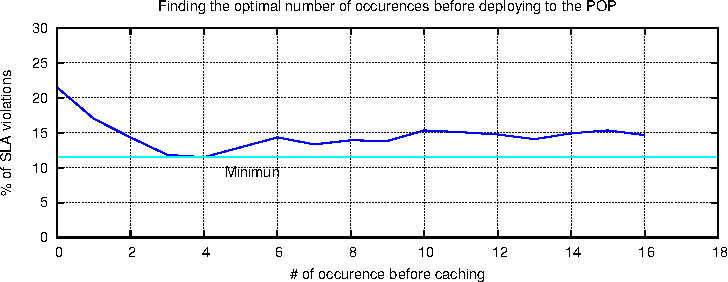
\includegraphics[width=0.45\textwidth]{fig/cachingStrat_evaluation.pdf}
  \end{center}
  \caption{ Caching Strategy Evaluation
    \label{fig:cachingstrateval}
  }
\end{figure}	

POP are designed to have great network performances for a given geographic area, and need to be spread throught the territory for a reduced price.
In order to mitigate the storage cost, the caching controller takes the decision to provision as few videos as possible to fullfill the SLA. Several factor can influence the decision, like the transcoding time, the vNF booting time, hosting costs and so on.
Taking the decision to provision a video in a specific POP means classifying the video as cachable according to some metadata, like the view count in a certain time window.
In \cite{silvestre_boosting_2015}, the authors proposed a model for predicting the popularity of a video, and estimated that view counts accounted for 82\% of the relative importance. 
We implemented a very simple provisionning policy, based on the number of requests for the same resource received in a 10 minutes rolling window. If the number is above the threshold, the video is cached at the POP level and clients can download the video from there.

~Figure \ref{fig:cachingstrateval} shows that for our particular settings, the option that minimize the percentage of SLA violation is 4. This can be explained by the fact that we want to preserve the POP for serving only the most popular videos (which will trigger the most SLA violations) and not clutter it with less popular videos that could be easily served by the CP. However, as the propagation of the caching policy takes time, we want to react promptly and not wait for too many popular videos to hitting the CP.

In production, this evaluation should be updated regularly by monitoring the overall traffic and the network conditions and possibly using other video metadata.





